\section{Hypothesis Testing}

  This was done for the first time as early as 1710, when a researcher tried to measure sex ratios in a population \cite{1710arbuthnot}. 
  
  A significance test is a method used to decide whether the data at hand sufficiently supports a particular hypothesis. The hypothesis to be tested is called the \textbf{alternative hypothesis}, denoted $H_1$ or $H_a$, and the status quo is called the \textbf{null hypothesis}, denoted $H_0$. Assuming that $H_0$ is true, we compute the likelihood of the data happening. If the sample is not too unlikely (past some significance level), we fail to reject $H_0$, and if there is strong evidence, we reject $H_0$. $H_0$ and $H_a$ can be devised in countless ways. 

  \begin{example}
    There are countless test statistics we can build, but here are some common examples, 
    \begin{enumerate}
      \item Proportion: Company A produces circuit boards, but 10\% of them are defective. Company B claims that they produce fewer defective circuit boards. 
      \begin{equation}
        H_0 : \, p = 0.10 \text{ versus } H_a : \, p < 0.10
      \end{equation}
      
      \item Means: It is known that the average height of boys in KIS is 176cm. Ben claims that the average height is lower than this. 
      \begin{equation}
        H_0 : \, \mu = 176 \text{ versus } H_a : \, \mu < 176
      \end{equation}
      
      \item Difference of Means: If $\mu_1$ and $\mu_2$ denote the true average breaking strengths of the same type of twine produced by two different companies. Jenny claims that the $\mu_1 - \mu_2 > 5$. 
      \begin{equation}
        H_0 : \, \mu_1 - \mu_2 = 0 \text{ versus } H_a : \, \mu_1 - \mu_2 > 5
      \end{equation}
    \end{enumerate}
  \end{example}

\subsection{Sampling Distributions}

  \begin{definition}[Population, Parameters]
    When conducting a statistical study, there is a set of items or events which is of interest for some experiment. This can be modeled with some probability space $(\Omega, \mathcal{F}, \mathbb{P})$. Usually, we are interested in some numerical property of this population, and so we implicitly define a random variable $X: \Omega \longrightarrow \mathbb{R}$ that induces some distribution $X \sim P$, which we call the \textbf{population}. A statistical population can be a group of existing objects or a hypothetical and potentially infinite group of objects conceived as a generalization from experience. 

    With this, we can interpret the population $X \sim P$ as a random variable, and we often call this the \textbf{parent distribution}. We are often interested in its population \textbf{parameters}, which can be any measured quantity of a population that summarizes or describes an aspect of it. In generality, the parameter of population $X$ is denoted $\theta$, and it is a fixed value. 
  \end{definition} 

  \begin{example}[Populations]
    Here are some examples of populations: 
    \begin{enumerate}
      \item We let $\Omega$ be the discrete sample space of all hands in poker, and our random variable will assign a numerical ranking to each hand $0$ for no hand, $1$ for pairs, $2$ for two pairs, etc. 
      \item $\Omega$ is the sample space of all individuals in the U.S. and we can construct a random variable $X$ that assigns to each individual their height. Even though $\Omega$ is finite, we can interpret it as continuous, which leads to a continuous distribution $X \sim P$. 
    \end{enumerate}
  \end{example}

  \begin{example}[Parameters]
    Some population parameters can be: 
    \begin{enumerate}
      \item The true mean of the population $\mu_X = \mathbb{E} [X]$
      \item The true variance of the population $\sigma^2_X = \Var[X]$ 
      \item In the height example, we can set $X = (X_1, X_2, X_3)$ and try to construct a linear regression model that predicts $X_3$ from $X_1, X_2$. Theoretically, this is $\mathbb{E}[X_3 \mid X_1, X_2]$, and we must find the best function of form $x_3 = a + b_1 x_1 + b_2 x_2$ that is closest to the conditional expectation. There does exist a unique one, and so $a, b_1, b_2$ are all population parameters. 
    \end{enumerate}
  \end{example}

  In general, the population is the total set of all relevant things that we are interested in. The specific quantity of the actual population is called the \textbf{population parameter}, e.g. the true mean $\mu$ or the true variance $\sigma^2$ of $X$, usually denoted with $\theta$. But usually, these parameters are not known since the population is too big to experimentally measure, so we must try and estimate it with samples. This is the entire point of statistics; otherwise, we would already know everything we want to know. 

  \begin{definition}[Samples]
    From the population $X \sim P$ (which still has unknown distribution), we can take $n$ \textbf{samples} by considering iid $x_1, x_2, \ldots, x_n \sim P$. 
    \begin{enumerate}
      \item We should note that the samples $x_i$ are random variables themselves. Not fixing them yet and still considering them in generality as random objects allows us to do more theoretical calculations. 
      \item Once these samples have been realized (i.e. $\omega \in \Omega$ is realized, and all $x_i$'s are also realized), we can treat them as fixed values. 
    \end{enumerate}
    Sometimes, we may not assume independence, but for most cases we do. A common rule is that if the sample size $n$ is less than 10\% of the population size, then we can assume independence. 
  \end{definition}

  \begin{definition}[Empirical Distribution]
    Now given that we have these iid samples, we can construct the \textbf{empirical distribution} $\widehat{X} \sim \widehat{P}$, defined as the discrete distribution that assigns probability $1/n$ to each value $x_i$ for $i \in [n]$. In other words, we have 
    \begin{equation}
      \mathbb{P}(\widehat{X} = x) = \frac{1}{n} \text{ for } x \in \{x_1, \ldots, x_n\}
    \end{equation}
    We can write the CDF of the empirical distribution, called the \textbf{empirical distribution function}, as the sum of indicators
    \begin{equation}
      F_X (x) = \frac{1}{n} \sum_{i=1}^n \mathbb{I}_{[x_i, +\infty)} (x)
    \end{equation}
  \end{definition}

  As expected, we would expect the empirical distribution to converge to the actual distribution. 

  \begin{theorem}[Glivenko–Cantelli theorem]
    The empirical distribution of iid samples $x_1, \ldots, x_n \sim P_n$ converges almost surely to $X \sim P$ as $n \rightarrow \infty$. More specifically, given that the CDF of $X$ is $F$ and the CDF of $P_n$ is the step function $F_n$, we have 
    \begin{equation}
      ||F_n - F||_{\infty} = \sup_{x \in \mathbb{R}} |F_n (x) - F(x)| \rightarrow 0
    \end{equation}
    almost surely as $n \rightarrow \infty$. 
  \end{theorem}

  \begin{example}[Empirical Distribution of Standard Gaussian]
    We expect the empirical distribution of the standard Gaussian to converge. Indeed, numerical results show that for 10 and 100 samples, the empirical CDF does converge to the true CDF. 

    \begin{center}
      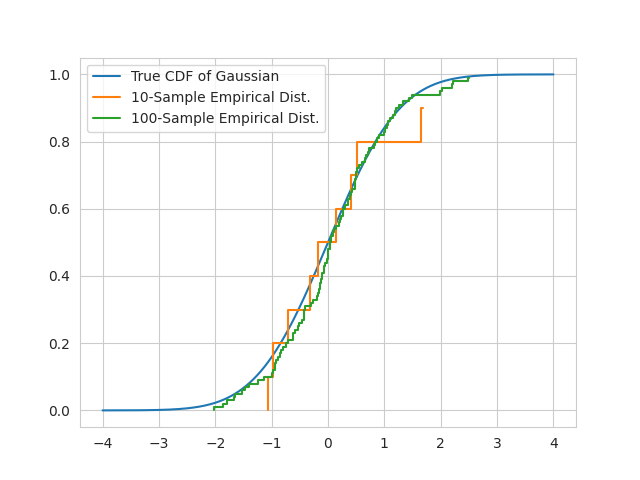
\includegraphics[scale=0.4]{img/empirical_distribution.png}
    \end{center}
  \end{example}

\subsection{Concentration of Measure}

  Now let's move on to concentration inequalities, which say that the probability that a random variable is greater than something is bounded by something. These probability bounds are extremely useful in of themselves. It allows us to talk about convergence theory, which tells us what happens to a statistic, such as $\overline{X}$, as I get more and more data. The first inequality exploits the fact that the tails of a Gaussian RV decay very quickly, and a lot of concentration inequalities attempt to mimic this exponential bound but for non-Gaussian distributions. 

  \begin{theorem}[Gaussian Tail Inequality]
  Given $X \sim \mathcal{N}(0, 1)$, the inequality says that the probability of $X$ taking values past a certain $t$ decays exponentially. 
  \[\mathbb{P} \big( |X| > t \big) \leq \frac{2 e^{-t^2/2}}{t}\]
  If we have $x_1, \ldots, x_n \sim \mathcal{N}(0, 1)$, then 
  \[\mathbb{P} \big( |\overline{X}| > t \big) \leq \frac{2}{\sqrt{n} t} e^{-n t^2/2}\]
  We can assume that the coefficient is less than $1$ if $n$ is large. The above tells us that this bound exponentially decays with $t$ but also with the number of samples $n$. 
  \end{theorem}

  \begin{theorem}[Markov's Inequality]
  Given a nonnegative random variable $X > 0$, we have 
  \[\mathbb{P}(X > t) \leq \frac{\mathbb{E}[X]}{t}\]
  \end{theorem}
  \begin{proof}
  We have 
  \begin{align*}
      \mathbb{E}[X] & = \int_0^\infty x p_X (x)\,dx \\
      & \geq \int_t^\infty x p_X (x) \,dx \\
      & = t \int_t^\infty p_X (x) \,dx \\
      & = t \mathbb{P}(X > t)
  \end{align*}
  \end{proof}

  \begin{theorem}[Chebyshev's Inequality]
  Given a random variable $X$ with mean $\mu = \mathbb{E}[X]$, we have 
  \[\mathbb{P}\big( |x - \mu| > t\big) \leq \frac{\mathrm{Var}(X)}{t^2}\]
  \end{theorem}

  \begin{theorem}[Hoeffding's Inequality]
  Let $x_1, x_2, \ldots, x_n$ be independent (not necessarily identical) random variables s.t. $a_i \leq X_i \leq b_i$ almost surely. Consider the random variable $\overline{X} = \frac{1}{n} (x_1 + \ldots + x_n)$. Then, for all $t > 0$, 
  \[\mathbb{P}\big( \big| \overline{X} - \mathbb{E}[\overline{X}] \big| \geq t \big) \leq 2 \exp \bigg( -\frac{2 n^2 t^2}{\sum_{i=1}^n (b_i - a_i)^2} \bigg)\]
  \end{theorem}

  Now in addition to bounding probabilities, we would like to bound expectations. 

  \begin{theorem}[Cauchy-Schwartz]
  Given random variables $X, Y$, it is often hard to compute the expectation of $X Y$ since it is hard to compute the distribution of it (sums are easy). But we can bound it as 
  \[|\mathbb{E}[XY]| \leq \mathbb{E}[ |XY| ] \leq \sqrt{\mathbb{E}[X] \, \mathbb{E}[Y]}\]
  \end{theorem}

  \begin{theorem}[Jensen's Inequality]
  Given $g$ a convex function and $X$ a random variable, we have 
  \[\mathbb{E}[ g(X)] \geq g (\mathbb{E}[X])\]
  \end{theorem}

  \subsection{Kullback Leibler Divergence}

  Now a popular metric between PMFs/PDFs is the KL divergence. 

  \begin{definition}[Kullback-Leibler Divergence]
  Given random variable $X$ and $Y$, 
  \begin{enumerate}
      \item If they are discrete with PMFs $P$ and $Q$, the KL-divergence is defined 
      \[D_{KL} (P \mid\mid Q) \coloneqq \sum_{x} P(x) \, \log \bigg(\frac{P(x)}{Q(x)} \bigg) = \mathbb{E} \bigg[ \log \frac{P(x)}{Q(x)} \bigg] \]
      where we can interpret the expectation as $X \sim p$. 
      \item If they are continuous with PDFs $p$ and $q$, the KL-divergence is defined 
      \[D_{KL} (p \mid\mid q) \coloneqq \int p(x) \, \log \bigg( \frac{p(x)}{q(x)} \bigg)\,dx = \mathbb{E} \bigg[ \log \frac{P(x)}{Q(x)} \bigg] \]
      where we can interpret the expectation as $X \sim p$. 
  \end{enumerate}
  \end{definition}

  \begin{enumerate}
      \item The fact that $D_{KL} (p \mid p) = 0$ is obvious. 
      \item To prove that $D_{KL} (p \mid q) \geq 0$, we use Jensen's inequality
      \[-D_{KL} (p \mid q) = \mathbb{E} \log \frac{q(X)}{p(X)} \leq \log \mathbb{E} \frac{q(X)}{p(X)} = \log \int \frac{q(x)}{p(x)} \, p(x) \, dx = \log(1) = 0\]
  \end{enumerate}
  This is not a metric though. 

  \subsection{Bounding Maximum of Random Variables}

  Given that we have $n$ samples $x_1, \ldots, x_n \sim P$, it is conventional to index them with open brackets to denote order 
  \[X_{(1)} \leq X_{(2)} \leq \ldots \leq X_{(n)}\]
  Our goal is now to find the distribution of $X_{(n)} = \max_i X_i$. If we know the distribution of $P$, $\mathbb{P}(X_{(n)} \leq x)$ is just the probability that all the $X_i$'s are less than $x$, and by independence we can product out the CDFs, differentiate to get the PDF, and compute. So it's not too hard to do this theoretically, but in practice this is hard to do since we don't exactly know $P$. 

  So if you didn't know the $X_i$'s, the best you can assume is that 
  \[\mathbb{E} \max\{x_1, \ldots, x_n\}\]
  is going to grow like $n$. But if we can bound the MGF with $\mathbb{E} e^{t X} \leq e^{t^2 \sigma^2}{2}$, then we can show that $\mathbb{E} \max X_i$ doesn't grow like $n$, but rather like $\log{n}$. 
  \[\mathbb{E} \max{X_i} \leq \sigma \sqrt{2 \log{n}}\]

  \subsection{Big-O, Little-O Notation}

  Going back to calculus, if we have a function $f: X \longrightarrow \mathbb{R}$, we can say that 
  \begin{enumerate}
      \item $f(x) = O(g(x))$ if $f$ is of the same order as $g$. That is, they grow at the same rate 
      \[\frac{f(x)}{g(x)} \rightarrow c \text{ as } x \rightarrow \infty\]
      for some constant $c$. 
      \item $f(x) = o(g(x))$ if $f$ is negligible w.r.t. $g$. That is, $f$ is infinitesimal w.r.t. $g$. 
      \[\frac{f(x)}{g(x)} \rightarrow 0 \text{ as } x \rightarrow \infty\]
      for some constant $c$. 
  \end{enumerate}
  Now there is a probabilistic notation as well. The concept of boundedness translates to being able to capture most of the mass of the random variable within some interval, and infinitesimality translates to the probability mass concentrating around $0$. 

  \begin{definition}[$O_p, o_p$ Notation]
  Let $x_1, x_2, \ldots $ be a sequence of random variables. 
  \begin{enumerate}
      \item $x_n = o_p (1)$ if 
      \[\mathbb{P}(|Y_n| > \epsilon) \rightarrow 0 \text{ as } n \rightarrow \infty\]
      for all $\epsilon > 0$. This means that $x_n$ gets more and more concentrated around $0$. 

      \item $x_n = O_p(1)$ if for all $\epsilon > 0$, then there exists a $C$ s.t. 
      \[\mathbb{P}(|x_n| > C) \leq \epsilon\]
      for all large $n$. That is, we can always trap the majority of the probability mass of $x_n$ within the interval $[-C, C]$. This must hold for all $x_n$ with $n > N$, so the mass can't "escape" to infinity. We can think of it as the distribution is "settling down" and not shooting off to somewhere. 

      \item $x_n = o_p (a_n)$ means that 
      \[\frac{x_n}{a_n} = o_p (1)\]

      \item $x_n = O_p (a_n)$ means that 
      \[\frac{x_n}{a_n} = O_p(1)\]
  \end{enumerate}
  \end{definition}

  \begin{theorem}
  Given $Y_1, \ldots Y_n \sim \mathrm{Bernoulli}(p)$, let $\widehat{p} = \frac{1}{n} \sum Y_i$. Then 
  \[\widehat{p}_n - p = o_p (1)\]
  which is also written $\widehat{p}_n = p + o_p (1)$, which means that the random variable $\widehat{p}_n$ is some constant $p$ plus a random variable that is going to $0$. 
  \end{theorem}
  \begin{proof}
  By Hoeffding's inequality, 
  \[\mathbb{P}(| \widehat{p}_n - p | > \epsilon) \leq 2 e^{-2n \epsilon^2}\]
  which goes to $0$ as $n \rightarrow \infty$. 
  \end{proof}

  \begin{example}
  Given $Y_1, \ldots Y_n \sim \mathrm{Bernoulli}(p)$, let $\widehat{p} = \frac{1}{n} \sum Y_i$. Then, 
  \[\widehat{p} - p = O_p \Big( \frac{1}{\sqrt{n}} \Big)\]
  \end{example}

\subsection{One Sample Z and T Tests}

  Let us have some population $X \sim P$ and a null hypothesis that claims $H_0 : \, \mu = \theta_0$. Since we are interested in the mean, we would like to use CLT or some other theorem to determine what the distribution of the mean of $n$ samples $\overline{x}_n$ looks like (either Normal or Student T centered around $\theta_0$ and scaled down by factor of $\sqrt{n}$). When we actually sample, the value $\overline{x}_n = \hat{\theta}$ is realized, and we would like to see if sampling $\hat{\theta}$ from the distribution centered around $\theta_0$ is likely, usually after normalizing. If it isn't, then we reject $H_0$. 

  How do we decide whether to use the z-test or the t-test? It is known that $\mathrm{StudentT}(n-1)$ converges to $\mathcal{N}(0, 1)$ in distribution as $n \rightarrow +\infty$. Therefore, depending on the context of the problem, at a certain point $N$ (usually $N = 30$ or perhaps higher for skewed distributions), the difference between these two are negligible. 
  \begin{enumerate}
    \item Z-test: if we know the population variance $\sigma^2$, but it is rarely the case that we actually know $\sigma^2$. 
    \item T-test: if we do not know the population variance $\sigma^2$, which we then substitute for the sample variance $S^2$. 
    \item Z-test: if we do not know the population variance (which we substitute for $S^2$), but our sample size is greater than $N$, then we can approximate the $t$-distribution with our normal, allowing us to use the Z-test again. 
  \end{enumerate}

  In general, the alternative to the null hypothesis $H_0 : \, \theta = \theta_0$ will looks like one of the following three assertions: 
  \begin{enumerate}
    \item Two-Sided Test: $H_a : \, \theta \neq \theta_0$ 
    \item One-Sided Test: $H_a : \, \theta > \theta_0$ (in which case the null hypothesis is $\theta \leq \theta_0$) 
    \item One-Sided Test: $H_a : \, \theta < \theta_0$ (in which case the null hypothesis is $\theta \geq \theta_0$) 
  \end{enumerate}

  Now we must still quantify \textit{how} unlikely our sample mean $\theta$ must be compared to $\theta_0$ in order to reject the null hypothesis. This is where we specify our \textbf{significance level}, denoted by $\alpha$ (common values $0.10, 0.05, 0.01$). This specifies the tail-regions in which $\theta$ will land in with probability $\alpha$. Usually, working with general normal/t distributions is tedious, so we can rescale them and use their z/t-scores. 

  \begin{definition}[Z-score]
    Given a value $x$ sampled from distribution $X \sim \mathcal{N}(\mu, \sigma^2)$, its \textbf{z-score} is defined to be the number of standard deviations away from the mean. 
    \begin{equation}
      z \coloneqq \frac{x - \mu}{\sigma}
    \end{equation}
    Now given a significance level $\alpha \in [0, 1]$, let $z_\alpha$ be the value such that the measure of a standard normal distribution past $z_\alpha$ is $1 - \alpha$ (i.e. the $100\alpha$ percentile). $z_\alpha$ is called the \textbf{critical z-value}.
  \end{definition}

  \begin{definition}[T-score]
    Given a value $x$ sampled from distribution $X \sim \mathrm{StudentT}(n)$, its \textbf{t-score} is defined to be the number of standard deviations away from the mean. 
  \end{definition}

  \begin{example}
    A factory has a machine that dispenses 80mL of fluid in a bottle. An employee believes the average amount of fluid is not 80mL. Using 40 samples, he measures the average amount dispensed by the machine to be 78mL with a sample standard deviation of 2.5. 
    \begin{enumerate}
      \item Let the true mean be $\mu$ and true standard deviation be $\sigma$. The null hypothesis is $H_0 : \, \mu = 80$ and the alternative is $H_1 : \, \mu \neq 80$, making this a two-sided test. 
      
      \item We don't know the true standard deviation $\sigma$, so we must use the sample standard deviation $S$. This requires us to use the $t$-test, but since $n > 30$, we can invoke CLT and state that $\overline{x}_{40}$ is (approximately) Gaussian with mean $\mu$ and standard deviation $S / \sqrt{n}$. So, we use the $z$-test. 
      
      \item At a 95\% confidence level, we have $\alpha = 0.05$, and our rejection region is $(-\infty, z_{0.025}] \cup [z_{0.975}, +\infty)$. Since we are looking at a standard Gaussian, we have by symmetry $z_{0.025} = -1.96$ and $z_{0.975} = 1.96$, and our critical z-value is $z^\ast = 1.96$. 
      
      \item So the z-score for $78$ is 
      \begin{equation}
        z = \frac{\overline{x} - \mu_0}{s / \sqrt{n}} = \frac{78 - 80}{2.5 / \sqrt{40}} = -5.06
      \end{equation}
      which is definitely in the reject region. So this tells us that we can reject the null hypothesis with a 95\% level of confidence. 
    \end{enumerate}
  \end{example}

  \begin{example}
    A company manufactures car batteries with an average life span of 2 or more years. An engineer believes this value to be less. Using 10 samples, he measures the average life span to be 1.8 years with a standard deviation of 0.15. 
    \begin{enumerate}
      \item Let the true mean be $\mu$ and true standard deviation be $\sigma$. The null hypothesis is $H_0: \, \mu \geq 2$ and the alternative is $H_1 : \, \mu < 2$, making this a one-sided test. 
      
      \item We don't know the true standard deviation $\sigma$, so we must use the sample standard deviation $S$. This requires us to use the $t$-test, especially since $n = 10$ is not large enough for us to invoke CLT. 
      
      \item At a 99\% confidence level, we have $\alpha = 0.01$, and our rejection region is $(-\infty, t_{0.01}] = (-\infty, -2.82]$. 
      
      \item The t-score for the observed mean value is 
      \begin{equation}
        t = \frac{\overline{x} - \mu_0}{s / \sqrt{n}} = \frac{1.8 - 2}{0.15 / \sqrt{10}} = -4.22
      \end{equation}
      which is definitely in the reject region. So this tells us that we can reject the null hypothesis with a 99\% level of confidence. 
    \end{enumerate}
  \end{example}

  We may have to account for errors. There is always a chance that our evidence leads us to an incorrect conclusion, and we have names for this. 

  \begin{definition}[Errors]
    Given a hypothesis test where we look for evidence supporting our alternative claim, 
    \begin{enumerate}
      \item A \textbf{type 1 error} is when the null hypothesis is rejected, but it is true (false positive). 
      \item A \textbf{type 2 error} is when we fail to reject the null hypothesis, when it is false (false negative). 
    \end{enumerate}
  \end{definition}

\subsection{Power of a test}

\subsection{Common tests (t-test, z-test, chi-square test, F-test)}

\subsection{Multiple testing problem}

